%!TEX TS-program = xelatex
\documentclass[]{shiltemann-cv}
\addbibresource{publications.bib}

\begin{document}
\header{Saskia}{Hiltemann}
       {Doctoral Researcher, Bioinformatics \& Training}


% In the aside, each new line forces a line break
\begin{aside}
  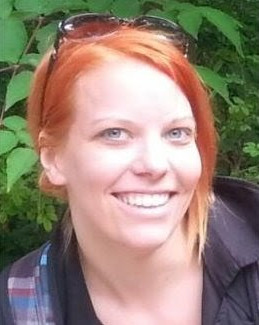
\includegraphics[width=75pt]{foto.jpg}
  \section{About}
    Laakkade 378
    2521 XV, Den Haag
    The Netherlands
    ~
    zazkia@gmail.com
  \section{Languages}
    Bilingual Dutch/English
    German \& French
  \section{Coding}
    Python, C, C++
\end{aside}

\section{Interests}

Bioinformatics, Training, Community Building, Genome Sequencing, Data Anlysis, Workflows, Automation, Visualisation, Best Practices, Cancer Research, Microbiome Analysis, Infosec, CTF, Traveling, Hiking, Reading, Puzzles.

\section{Education}

\begin{entrylist}
  \entry
    {Since 2012}
    {Ph.D. {\normalfont candidate in Bioinformatics}}
    {Erasmus Medical Center}
    {\emph{Bioinformatics for Everybody.}}
  \entry
    {2008–2010}
    {M.Sc.}
    {LIACS, University of Leiden \& TU Delft}
    {Computer Science\\
    Specialization in Bioinformatics}
  \entry
    {2005–2008}
    {B.Sc.}
    {LIACS, University of Leiden}
    {Computer Science}
  \entry
    {2002–2005}
    {B.Sc. course work}
    {University of Leiden}
    {Physics \& Astronomy}
  \entry
    {2002}
    {High School (VWO)}
    {Alfrink College, Zoetermeer}
    {Specialization in Science \& Technology}
\end{entrylist}

\section{Work Experience}

\begin{entrylist}
 \entry
    {Current}
    {Erasmus Medical Center, Rotterdam}
    {}
    {Bioinformatician and Doctoral Researcher
     \begin{itemize}
     \item \emph{Software Development and Pipeline building}
     \item \emph{Training Development and Delivery}
     \item \emph{Galaxy System's Administrator}
     \item \emph{Microbiota Analysis and Antibiotic Resistance Detection}
     \item \emph{Prostate Cancer Analysis}
     \end{itemize}}
  \entry
    {2010-2012}
    {After's Cool, The Hague}
    {Tutor of High School Students.}
    {Tutor of High School Students. \emph{Math, Physics, Chemistry}}
  \entry
    {2002-2010}
    {Self-Employed}
    {}
    {Tutor of High School Students. \emph{Math, Physics, Chemistry}}
\end{entrylist}

\section{Projects}

\begin{entrylist}
  \entry
    {2018}
    {Clinical Microbiota Analysis Pipeline}
    {ErasmusMC}
    {Development of an analysis pipeline for use in daily clinical diagnostics of sepsis patients for Streeklab Haarlem.}
  \entry
    {2016-18}
    {Galaxy Training Materials}
    {GalaxyProject}
    {Co-developed infrastructure for the collaborative development of Galaxy training materials, as well as development of several training manuals on topic of Metagenomics, Galaxy Development and Visualisation}
\end{entrylist}

\newpage
\newgeometry{left=3cm}

\begin{entrylist}
  \entry
    {2016}
    {Galaxy CTF}
    {Galaxy Community Conference 2016}
    {Together with Helena Rasche, built a framework and 28 challenges for a “Capture the Flag” event based on Galaxy. Tasks included exploiting recently patched security bugs within Galaxy, Docker security issues, exploring new Galaxy features, and exploiting common bugs in Galaxy tools. Approximately 16 people participated in the competition. The infrastructure for the competition was released afterwards to allow others to re-use it for educational purposes.}

\end{entrylist}

\section{Publications}


\begin{enumerate}
\item MYcrobiota

\item Training materials

\item Galaxy update

\item ASAIM

\item Chao Zhang, Jochem Bijlard, Christine Staiger, Serena Scollen4, David van Enckevort, Youri Hoogstrate, Alexander Senf, \textbf{Saskia Hiltemann}, Susanna Repo, Wibo Pipping, Mariska Bierkens, Stefan Payralbe, Bas Stringer, Jaap Heringa, Andrew Stubbs, Luiz Olavo Bonino Da Silva Santos, Jeroen Belien, Ward Weistra, Rita Azevedo, Kees van Bochove, Gerrit Meijer, Jan-Willem Boiten, Jordi Rambla, Remond Fijneman, J. Dylan Spalding, Sanne Abeln. {\color{lightgray}{Systematically linking tranSMART, Galaxy and EGA for reusing human translational research data.}}  \textit{F1000Research.} 2017, 6:1488 (doi: 10.12688/f1000research.12168.1).

\item Youri Hoogstrate, Chao Zhang, Alexander Senf, Jochem Bijlard, \textbf{Saskia Hiltemann}, David van Enckevort, Susanna Repo, Jaap Heringa, Guido Jenster, Remond J.A. Fijneman, Jan-Willem Boiten, Gerrit A. Meijer, Andrew Stubbs, Jordi Rambla, Dylan Spalding and Sanne Abeln. {\color{lightgray}{Integration of EGA secure data access into Galaxy.}}  \textit{F1000Research.} 2016;5:ELIXIR-2841. doi:10.12688/f1000research.10221.1.

\item Hoogstrate Y, Böttcher R, \textbf{Hiltemann S}, van der Spek PJ, Jenster G, Stubbs AP. {\color{lightgray}{FuMa: reporting overlap in RNA-seq detected fusion genes.}} \textit{Bioinformatics.} 2016 Apr 15;32(8):1226-8. doi: 10.1093/bioinformatics/btv721.

\item \textbf{Hiltemann S}, Jenster G, Trapman J, van der Spek P, Stubbs A. {\color{lightgray}{Discriminating somatic and germline mutations in tumor DNA samples without matching normals.}} \textit{Genome Research.} 2015;25(9):1382-1390. doi:10.1101/gr.183053.114.

\item Moorhouse MJ, van Zessen D, IJspeert H, \textbf{Hiltemann S}, Horsman S, van der Spek PJ, van der Burg M, Stubbs AP. {\color{lightgray}{ImmunoGlobulin galaxy (IGGalaxy) for simple determination and quantitation of immunoglobulin heavy chain rearrangements from NGS.}} \textit{BMC Immunology.} 2014;15:59. doi:10.1186/s12865-014-0059-7.

\item \textbf{Hiltemann S}, Hoogstrate Y, der Spek P van, Jenster G, Stubbs A. {\color{lightgray}{iReport: a generalised Galaxy solution for integrated experimental reporting.}} \textit{GigaScience.} 2014;3:19. doi:10.1186/2047-217X-3-19.

\item Teles Alves I, Hartjes T, McClellan E, \textbf{Hiltemann S}, Böttcher R, Dits N, Temanni MR, Janssen B, van Workum W, van der Spek P, Stubbs A, de Klein A, Eussen B, Trapman J, Jenster G. {\color{lightgray}{Next-generation sequencing reveals novel rare fusion events with functional implication in prostate cancer.}} \textit{Oncogene.} 2015 Jan 29;34(5):568-77. doi: 10.1038/onc.2013.591.

\item \textbf{Hiltemann S}, Mei H, de Hollander M, et al. {\color{lightgray}{CGtag: complete genomics toolkit and annotation in a cloud-based Galaxy.}} \textit{GigaScience.} 2014;3:1. doi:10.1186/2047-217X-3-1.

\item Teles Alves I, \textbf{Hiltemann S}, Hartjes T, van der Spek P, Stubbs A, Trapman J, Jenster G. {\textcolor{red}{Gene fusions by chromothripsis of chromosome 4q in the VCaP prostate cancer cell line.}} \textit{Hum Genet.} 2013 Jun;132(6):709-13. doi: 10.1007/s00439-013-1308-1.

\item \textbf{Hiltemann S}, McClellan EA, van Nijnatten J, Horsman S, Palli I, Teles Alves I, Hartjes T, Trapman J, van der Spek P, Jenster G, Stubbs A. {\color{lightgray}{iFUSE: integrated fusion gene explorer.}} \textit{Bioinformatics.} 2013 Jul 1;29(13):1700-1. doi: 10.1093/bioinformatics/btt252.

\item Stubbs A, McClellan EA, Horsman S, \textbf{Hiltemann S}, Palli I, Nouwens S, Koning AHJ, Hoogland F, Reumers J, Heijsman D, Swagemakers S, Kremer A, Meijerink J, Lambrechts D, van der Spek PJ. \textcolor{orange}{Huvariome: a web server resource of whole genome next-generation sequencing allelic frequencies to aid in pathological candidate gene selection.} \textit{Journal of Clinical Bioinformatics.} 2012;2:19. doi:10.1186/2043-9113-2-19.


\end{enumerate}

\section{Training}

%%% This piece of code has been commented by Karol Kozioł due to biblatex errors.
%
%\printbibsection{article}{article in peer-reviewed journal}
%\begin{refsection}
%  \nocite{*}
%  \printbibliography[sorting=chronological, type=inproceedings, title={international peer-reviewed conferences/proceedings}, notkeyword={france}, heading=subbibliography]
%\end{refsection}
%\begin{refsection}
%  \nocite{*}
%  \printbibliography[sorting=chronological, type=inproceedings, title={local peer-reviewed conferences/proceedings}, keyword={france}, heading=subbibliography]
%\end{refsection}
%\printbibsection{misc}{other publications}
%\printbibsection{report}{research reports}

\end{document}
